\section{Entwurf}

\begin{bonus}{Bestandteile einer Softwarearchitektur}
    \begin{itemize}
        \item Anwendungsspezifische Funktionen (Applikationslogik)
        \item Details der Benutzerschnittstelle (GUI-Bibliotheken)
        \item Ablaufsteuerung (Transaktionen, Workflowmanagement)
        \item Datenhaltung (in Dateien, Datenbanken)
        \item Infrastrukturdienste für
              \begin{itemize}
                  \item Objektverwaltung (Freispeichersammlung, verteilte Objekte)
                  \item Prozesskommunikation
              \end{itemize}
        \item Sicherheitsfunktionen (Verschlüsselung, Passwortschutz)
        \item Zuverlässigkeitsfunktionen (Fehlererkennung und -behebung)
        \item Systemadministration (Statistiken, Installation, Sicherung)
        \item Weitere Basisbibliotheken (arithmetische Funktionen)
        \item \ldots
    \end{itemize}
\end{bonus}

\begin{bonus}{Funktion der Architektur im Software-Lebenszyklus}
    \begin{tabularx}{\textwidth}{|>{\bfseries}l|>{- }X|}
        \hline
        Bauplan             & Spezifikation des zu implementierenden Systems sowohl auf grober als auch auf feiner Ebene   \\
        \hline
        Projektplanung      & Definition von Arbeitspaketen zum Implementieren und Testen                                  \\
                            & Definition von Meilensteinen                                                                 \\
                            & Aufteilung des Projektteams nach Architekturkomponenten                                      \\
                            & Fortschrittskontrolle                                                                        \\
        \hline
        Testen              & Festlegung von Teststrategien                                                                \\
                            & Ableitung von Testfällen                                                                     \\
        \hline
        Nachvollziehbarkeit & Management von Beziehungen zu Anwendungsfällen bzw. Funktionen der Anforderungsspezifikation \\
        \hline
        Wartung             & Verstehen des Systems                                                                        \\
                            & Analyse der Auswirkung von Änderungen                                                        \\
                            & Planung von Änderungen                                                                       \\
        \hline
    \end{tabularx}
\end{bonus}

\subsection{Entwurfsmuster}

\begin{defi}{Entwurfsmuster}
    \emph{Entwurfsmuster} sind bewährte Lösungsschablonen für wiederkehrende Entwurfsprobleme sowohl in der Architektur als auch in der Softwarearchitektur und -entwicklung.

    Sie stellen damit eine wiederverwendbare Vorlage zur Problemlösung dar, die in einem bestimmten Zusammenhang einsetzbar ist.

    Es gibt verschiedene Typen von Entwurfsmustern.
    Es werden folgende Typen unterschieden:
    \begin{itemize}
        \item \emph{Erzeugungsmuster (Creational Patterns)}:
              Dienen der Erzeugung von Objekten. Sie entkoppeln die Konstruktion eines Objekts von seiner Repräsentation.
              \begin{itemize}
                  \item Fabrikmethode (Factory method)
                  \item Abstrakte Fabrik (Abstract Factory)
                  \item Erbauer (Builder)
                  \item Prototyp (Prototype)
                  \item Singleton
              \end{itemize}
        \item \emph{Strukturmuster (Structural Patterns)}:
              Erleichtern den Entwurf von Software durch vorgefertigte Schablonen für Beziehungen zwischen Klassen.
              \begin{itemize}
                  \item Schablonenmethode (Template method)
                  \item Beobachter (Observer)
                  \item Iterator
                  \item Besucher (Visitor)
                  \item Strategie (Strategy)
                  \item Zustand (State)
              \end{itemize}
        \item \emph{Verhaltensmuster (Behavioral Patterns)}:
              Modellieren komplexes Verhalten der Software und erhöhen damit die Flexibilität der Software hinsichtlich ihres Verhaltens.
              \begin{itemize}
                  \item Stellvertreter (Proxy)
                  \item Kompositum (Composite)
                  \item Fassade (Facade)
                  \item Dekorierer (Decorator)
              \end{itemize}
    \end{itemize}
\end{defi}

\subsubsection{Verhaltensmuster}

\begin{defi}{Strategie-Muster}
    Das \emph{Strategie- (Strategy) Muster} ist im Bereich der Softwareentwicklung ein Entwurfsmuster und gehört zur Kategorie der Verhaltensmuster.

    Eine Strategie definiert eine Familie (zur Laufzeit) austauschbarer Algorithmen.

    \begin{center}
        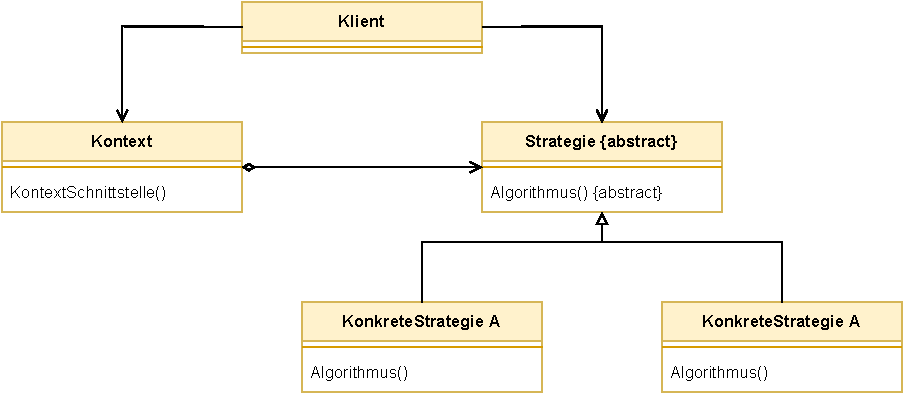
\includegraphics[width=0.9\textwidth]{includes/figures/defi_strategie.pdf}
    \end{center}
\end{defi}

\begin{example}{Strategie-Muster}
    % Wir definieren zuerst das Strategie-Interface \texttt{CatchStrategy} und zwei Implementierungen \texttt{PokeBallCatchStrategy} und \texttt{MasterBallStrategy}:
    \lstinputlisting[language=java]{includes/code/CatchStrategy.java}

    % Dann definieren wir einen Klienten, der eine beliebige Strategie verwendet:
    \lstinputlisting[language=java]{includes/code/Ball.java}

    % Die Verwendung sieht dann z.B. so aus:
    \lstinputlisting[language=java]{includes/code/StrategyExample.java}
\end{example}


\begin{defi}{Beobachter-Muster}
    Das \emph{Beobachter- (Observer) Muster} ist im Bereich der Softwareentwicklung ein Entwurfsmuster und gehört zur Kategorie der Verhaltensmuster.

    Ein Beobachter dient der Weitergabe von Änderungen an einem Objekt an von diesem Objekt abhängige Strukturen.

    \begin{center}
        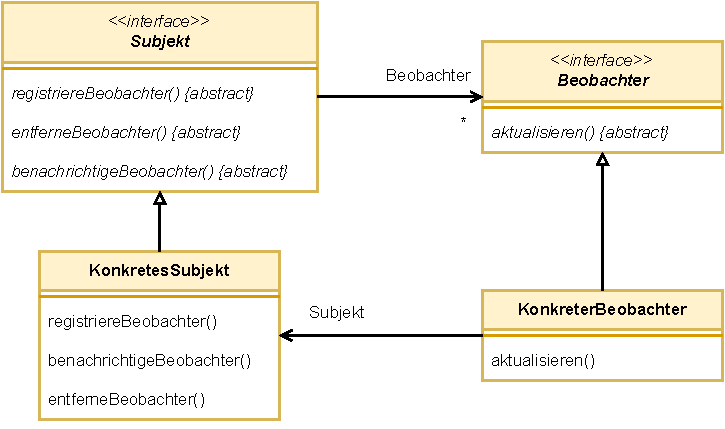
\includegraphics[width=0.7\textwidth]{includes/figures/defi_beobachter.pdf}
    \end{center}
\end{defi}

\begin{example}{Beobachter-Muster}
    % Zuerst definieren wir die Klasse \texttt{BattleNews} und die Klasse \texttt{Trainer} als Beobachter:
    \lstinputlisting[language=java]{includes/code/BattleNews.java}

    % Danach definieren wir die \texttt{NewsChannel} Klasse, die abonniert werden soll:
    \lstinputlisting[language=java]{includes/code/NewsChannel.java}

    % Die Verwendung sieht dann z.B. so aus:
    \lstinputlisting[language=java]{includes/code/BeobachterExample.java}
\end{example}

\begin{defi}{Zustand-Muster}
    Das \emph{Zustand- (State) Muster} ist im Bereich der Softwareentwicklung ein Entwurfsmuster und gehört zur Kategorie der Verhaltensmuster.

    Das Zustandsmuster wird zur Kapselung unterschiedlicher, zustandsabhängiger Verhaltensweisen eines Objektes eingesetzt.

    \begin{center}
        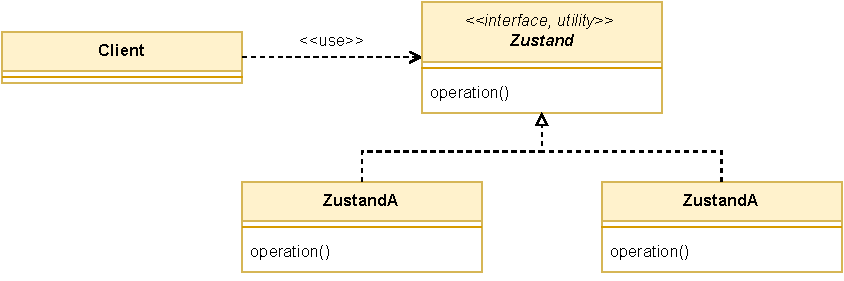
\includegraphics[width=0.9\textwidth]{includes/figures/defi_zustand.pdf}
    \end{center}
\end{defi}

\begin{example}{Zustand-Muster}
    \lstinputlisting[language=java]{includes/code/StatusCondition.java}

    \lstinputlisting[language=java]{includes/code/BattlePokemon.java}

    \lstinputlisting[language=java]{includes/code/StateExample.java}
\end{example}

\subsubsection{Erzeugungsmuster}

\begin{defi}{Singleton-Muster}
    Das \emph{Singleton Muster} ist im Bereich der Softwareentwicklung ein Entwurfsmuster und gehört zur Kategorie der Erzeugungsmuster.

    Es stellt sicher, dass von einer Klasse genau ein Objekt existiert.
    Dieses Singleton ist darüber hinaus üblicherweise global verfügbar.

    \begin{center}
        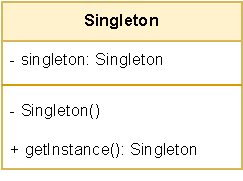
\includegraphics[width=0.3\textwidth]{includes/figures/defi_singleton.pdf}
    \end{center}
\end{defi}

\begin{example}{Singleton-Muster}
    Das Team der bzw. des ProtagonistIn des Spiels soll nur einmal existieren.

    Wir nutzen dafür ein Singleton-Muster wie folgt:
    \lstinputlisting[language=java]{includes/code/Team.java}

    \lstinputlisting[language=java]{includes/code/SingletonExample.java}
\end{example}

\begin{defi}{Fabrikmethode}
    Die \emph{Fabrikmethode (Factory Method)} ist im Bereich der Softwareentwicklung ein Entwurfsmuster und gehört zur Kategorie der Erzeugungsmuster.

    Das Muster beschreibt, wie ein Objekt durch Aufruf einer Methode anstatt durch direkten Aufruf eines Konstruktors erzeugt wird.

    \begin{center}
        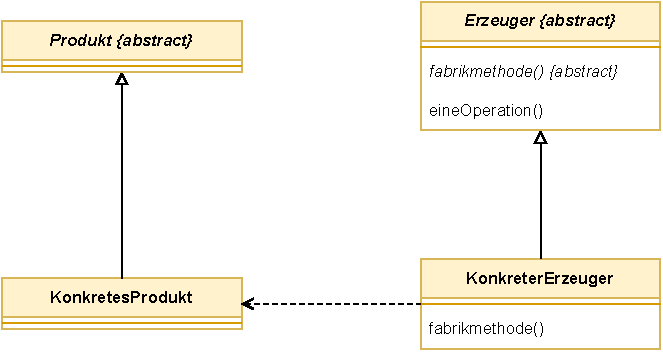
\includegraphics[width=0.7\textwidth]{includes/figures/defi_fabrikmethode.pdf}
    \end{center}
\end{defi}

\begin{example}{Fabrikmethode}

    \lstinputlisting[language=java]{includes/code/Trainer.java}

    \lstinputlisting[language=java]{includes/code/Gym.java}

    \lstinputlisting[language=java]{includes/code/FactoryExample.java}
\end{example}

\begin{defi}{Erbauer-Muster}
    Das \emph{Erbauer- (Builder) Muster} ist im Bereich der Softwareentwicklung ein Entwurfsmuster und gehört zur Kategorie der Erzeugungsmuster.

    Das Muster trennt die Konstruktion komplexer Objekte von deren Repräsentationen, wodurch dieselben Konstruktionsprozesse wiederverwendet werden können.

    Der Einsatz des Erbauer-Entwurfsmusters bietet sich an, wenn
    \begin{itemize}
        \item zu einem komplexen Objekt unterschiedliche Repräsentationen existieren sollen,
        \item die Konstruktion eines komplexen Objekts unabhängig von der Erzeugung der Bestandteile sein soll oder
        \item der Konstruktionsablauf einen internen Zustand erfordert, der vor einem Klienten verborgen werden soll.
    \end{itemize}

    \begin{center}
        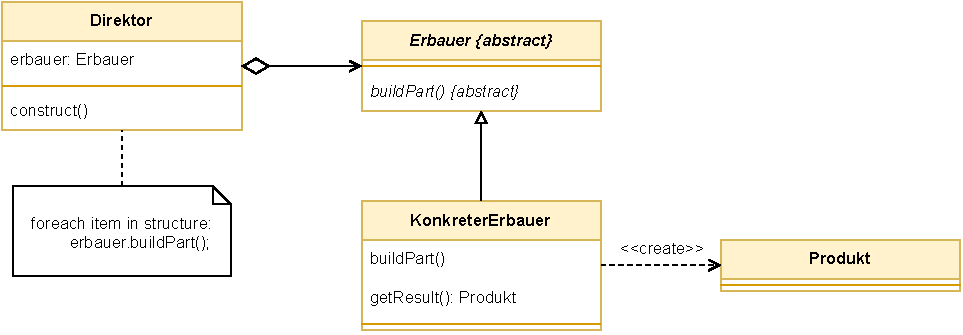
\includegraphics[width=0.7\textwidth]{includes/figures/defi_erbauer.pdf}
    \end{center}
\end{defi}


\begin{example}{Erbauer-Muster}
    %\lstinputlisting[language=java]{includes/code/Pokemon.java}

    \lstinputlisting[language=java]{includes/code/PokemonBuilder.java}

    \lstinputlisting[language=java]{includes/code/BuilderExample.java}
\end{example}

\subsubsection{Strukturmuster}

\begin{defi}{Fassade-Muster}
    Das \emph{Fassade- (Facade) Muster} ist im Bereich der Softwareentwicklung ein Entwurfsmuster und gehört zur Kategorie der Strukturmuster.

    Es bietet eine einheitliche und meist vereinfachte Schnittstelle zu einer Menge von Schnittstellen eines Subsystems.

    Wenn ein Subsystem viele technisch orientierte Klassen enthält, die selten von außen verwendet werden, hilft es, eine Fassade zu verwenden. Die Fassade ist eine Klasse mit ausgewählten Methoden, die eine häufig benötigte Untermenge an Funktionalität des Subsystems umfasst. Sie delegiert die Funktionalität an andere Klassen des Subsystems und vereinfacht dadurch den Umgang mit dem Subsystem.

    \begin{center}
        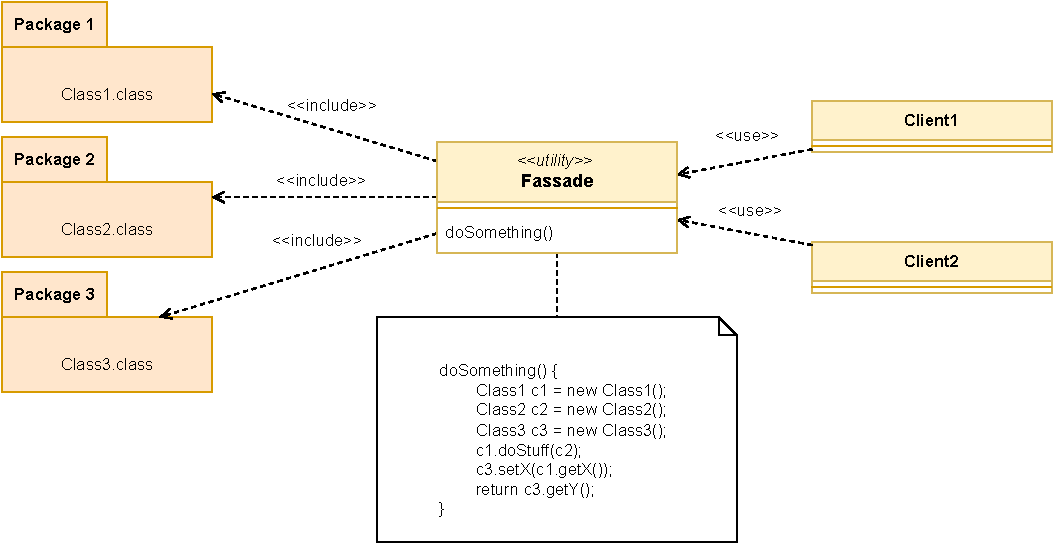
\includegraphics[width=0.9\textwidth]{includes/figures/defi_fassade.pdf}
    \end{center}
\end{defi}

\begin{example}{Fassade-Muster}

    \lstinputlisting[language=java]{includes/code/PokemonCenter.java}

    \lstinputlisting[language=java]{includes/code/Nurse.java}

    \lstinputlisting[language=java]{includes/code/FacadeExample.java}
\end{example}

\begin{defi}{Dekorierer-Muster}
    Das \emph{Dekorierer- (Decorator) Muster} ist im Bereich der Softwareentwicklung ein Entwurfsmuster und gehört zur Kategorie der Strukturmuster.

    Das Muster ist eine flexible Alternative zur Unterklassenbildung, um eine Klasse um zusätzliche Funktionalitäten zu erweitern.

    \begin{center}
        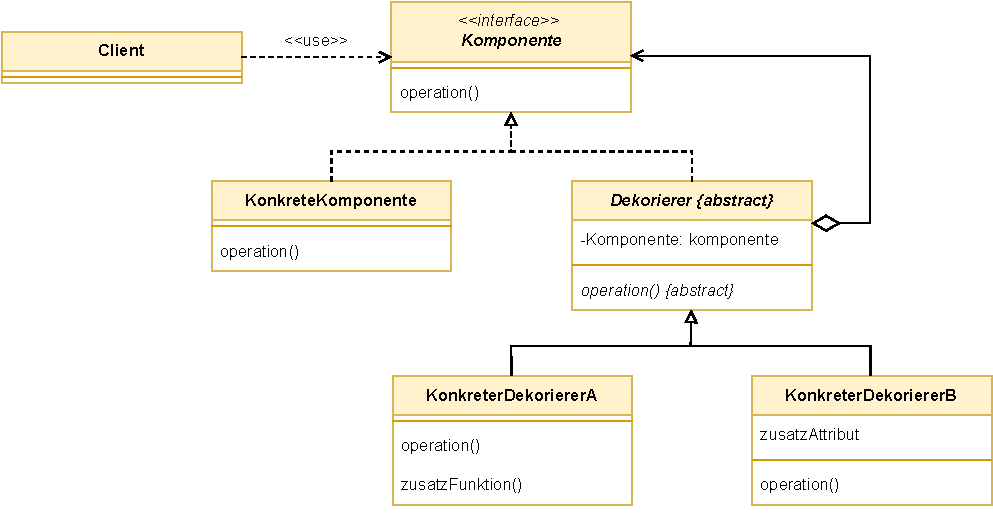
\includegraphics[width=0.9\textwidth]{includes/figures/defi_dekorierer.pdf}
    \end{center}
\end{defi}

\begin{example}{Dekorierer-Muster}

    \lstinputlisting[language=java]{includes/code/ContestPokemon.java}

    \lstinputlisting[language=java]{includes/code/DecoratorExample.java}
\end{example}

\begin{defi}{Kompositum-Muster}
    Das \emph{Kompositum- (Composite) Muster} ist im Bereich der Softwareentwicklung ein Entwurfsmuster und gehört zur Kategorie der Strukturmuster.

    Es ird angewendet, um Teil-Ganzes-Hierarchien zu repräsentieren, indem Objekte zu Baumstrukturen zusammengefügt werden.
    Die Grundidee des Kompositionsmusters ist, in einer abstrakten Klasse sowohl primitive Objekte als auch ihre Behälter zu repräsentieren.

    Somit können sowohl einzelne Objekte als auch ihre Kompositionen einheitlich behandelt werden.

    \begin{center}
        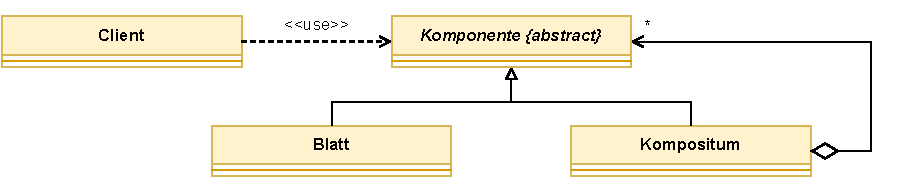
\includegraphics[width=0.9\textwidth]{includes/figures/defi_kompositum.pdf}
    \end{center}
\end{defi}

\begin{example}{Kompositum-Muster}
    \lstinputlisting[language=java]{includes/code/PokemonLeague.java}

    \lstinputlisting[language=java]{includes/code/CompositeExample.java}
\end{example}

\subsection{Architekturmuster}

\begin{defi}{Architekturmuster}
    Im Bereich der Softwareentwicklung sind \emph{Architekturmuster} in den Arten von Mustern auf oberster Ebene einzuordnen.

    Im Gegensatz zu Entwurfsmustern bestimmen sie nicht ein konkretes (meist kleines oder lokales) Teilproblem, sondern die grundlegende Organisation und Interaktion zwischen den Komponenten einer Anwendung.

    Architekturmuster lassen sich in verschiedene Kategorien einteilen:
    \begin{itemize}
        \item \textbf{Adaptive Systeme}:
              \begin{itemize}
                  \item Plug-In Architektur für Frameworks
              \end{itemize}
        \item \textbf{Struktur}:
              \begin{itemize}
                  \item EVA, Hollywood
                  \item ISO/OSI-Schichtenmodell
                  \item Pipes und Filter
                  \item Komponentenbasierte Architektur
                  \item Objektorientierte Architektur
              \end{itemize}
        \item \textbf{Interaktive Systeme}:
              \begin{itemize}
                  \item Model-View-Controller
                  \item Model-View-ViewModel
              \end{itemize}
        \item \textbf{Verteilte Systeme}:
              \begin{itemize}
                  \item Client-Server Architektur
                  \item N-Tier
                  \item Serviceorientierte Architektur
              \end{itemize}
    \end{itemize}
\end{defi}

\begin{defi}{Schichten-Muster}
    \begin{wrapfigure}{r}{0.2\textwidth}
        \centering
        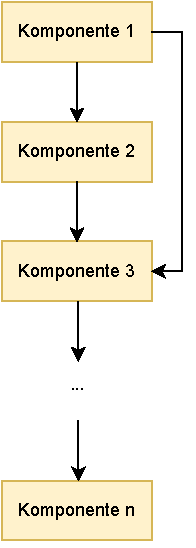
\includegraphics[width=0.15\textwidth]{includes/figures/defi_schichten.pdf}
    \end{wrapfigure}
    %
    Das \emph{Schichten-Muster} ist ein häufig angewandtes Strukturierungsprinzip für die Architektur von Softwaresystemen.
    Dabei werden einzelne Aspekte des Softwaresystems konzeptionell einer Schicht zugeordnet.

    Die erlaubten Abhängigkeitsbeziehungen zwischen den Aspekten werden bei einer Schichtenarchitektur dahingehend eingeschränkt, dass Aspekte einer höheren Schicht nur solche tieferer Schichten verwenden dürfen.

    Die den Schichten zugeordneten Aspekte können dabei je nach Art des Systems oder Detaillierungsgrad der Betrachtung (Funktionalitäten, Komponenten, Klassen, etc.) sein.

    \vspace{5em}
\end{defi}

\begin{defi}{Pipes und Filter}
    \emph{Pipes und Filter}  ist ein Architekturmuster aus dem Bereich der Softwareentwicklung. Es beschreibt die Struktur für Systeme, die Datenströme verarbeiten.

    Ein \emph{Filter} ist ein Verarbeitungsschritt.
    Jeder Filter hat eine Dateneingabe und eine Datenausgabe.
    In jedem Verarbeitungsschritt werden die einkommenden Daten umgewandelt.
    Bei der Umwandlung können den Daten Teile entnommen, hinzugefügt oder auch vollständig ersetzt werden.
    Die Art der Umwandlung wird durch den Filter bestimmt.

    Eine \emph{Pipe} stellt eine Verbindung zwischen den einzelnen Verarbeitungsschritten dar.

    \begin{center}
        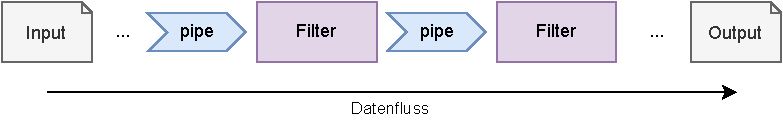
\includegraphics[width=0.9\textwidth]{includes/figures/defi_pipes_und_filter.pdf}
    \end{center}
\end{defi}

\begin{defi}{Model-View-Controller}
    \emph{Model-View-Controller}  ist ein Muster zur Unterteilung einer Software in die drei Komponenten \emph{Model}, \emph{View} und \emph{Controller}.
    Das Muster kann sowohl als Architekturmuster als auch als Entwurfsmuster eingesetzt werden.

    Ziel des Musters ist ein flexibler Programmentwurf, der eine spätere Änderung oder Erweiterung erleichtert und eine Wiederverwendbarkeit der einzelnen Komponenten ermöglicht.
    Die Umsetzungen nutzen dasselbe Model, nur Controller und View müssen dabei jeweils neu implementiert werden.

    Das \emph{Model} enthält Daten, die von der Präsentation dargestellt werden.
    Es ist von View und Controller unabhängig.

    Die \emph{View} ist für die Darstellung der Daten des Models und die Realisierung der Benutzerinteraktionen zuständig.
    Sie kennt das Model, dessen Daten sie präsentiert, ist aber nicht für die Verarbeitung dieser Daten zuständig.
    Des Weiteren ist sie von dem Controller unabhängig.

    Der \emph{Controller} verwaltet die View und das Model.
    Er wird von der View über Benutzerinteraktionen informiert, wertet diese aus und nimmt daraufhin Anpassungen an der View sowie Änderungen an den Daten im Model vor.

    \begin{center}
        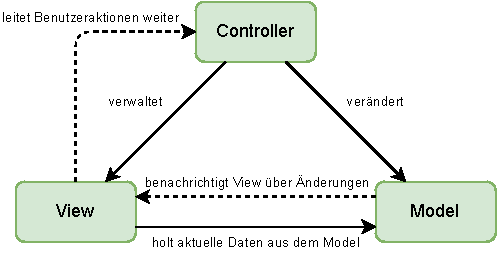
\includegraphics[width=0.7\textwidth]{includes/figures/defi_mvc.pdf}
    \end{center}
\end{defi}

\begin{defi}{Client-Server-Modell}
    Das \emph{Client-Server-Modell} beschreibt eine Möglichkeit, Aufgaben und Dienstleistungen innerhalb eines Netzwerkes zu verteilen.

    Die Aufgaben werden von Programmen erledigt, die in \emph{Clients} und \emph{Server} unterteilt werden.

    Der \emph{Client} kann auf Wunsch einen Dienst vom Server anfordern (z. B. ein Betriebsmittel).

    Der \emph{Server}, der sich auf demselben oder einem anderen Rechner im Netzwerk befindet, beantwortet die Anforderung (das heißt, er stellt im Beispiel das Betriebsmittel bereit); üblicherweise kann ein Server gleichzeitig für mehrere Clients arbeiten.

    \begin{center}
        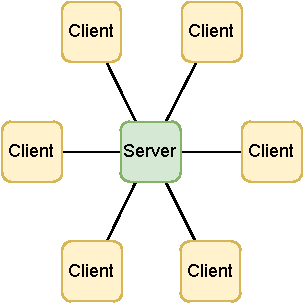
\includegraphics[width=0.4\textwidth]{includes/figures/defi_client_server.pdf}
    \end{center}
\end{defi}